\section{Question-only replay with Attention Distillation (\qstmethodshort{})}
\input{sec/setting}
\label{sec:method}

\begin{figure*}
    \centering
    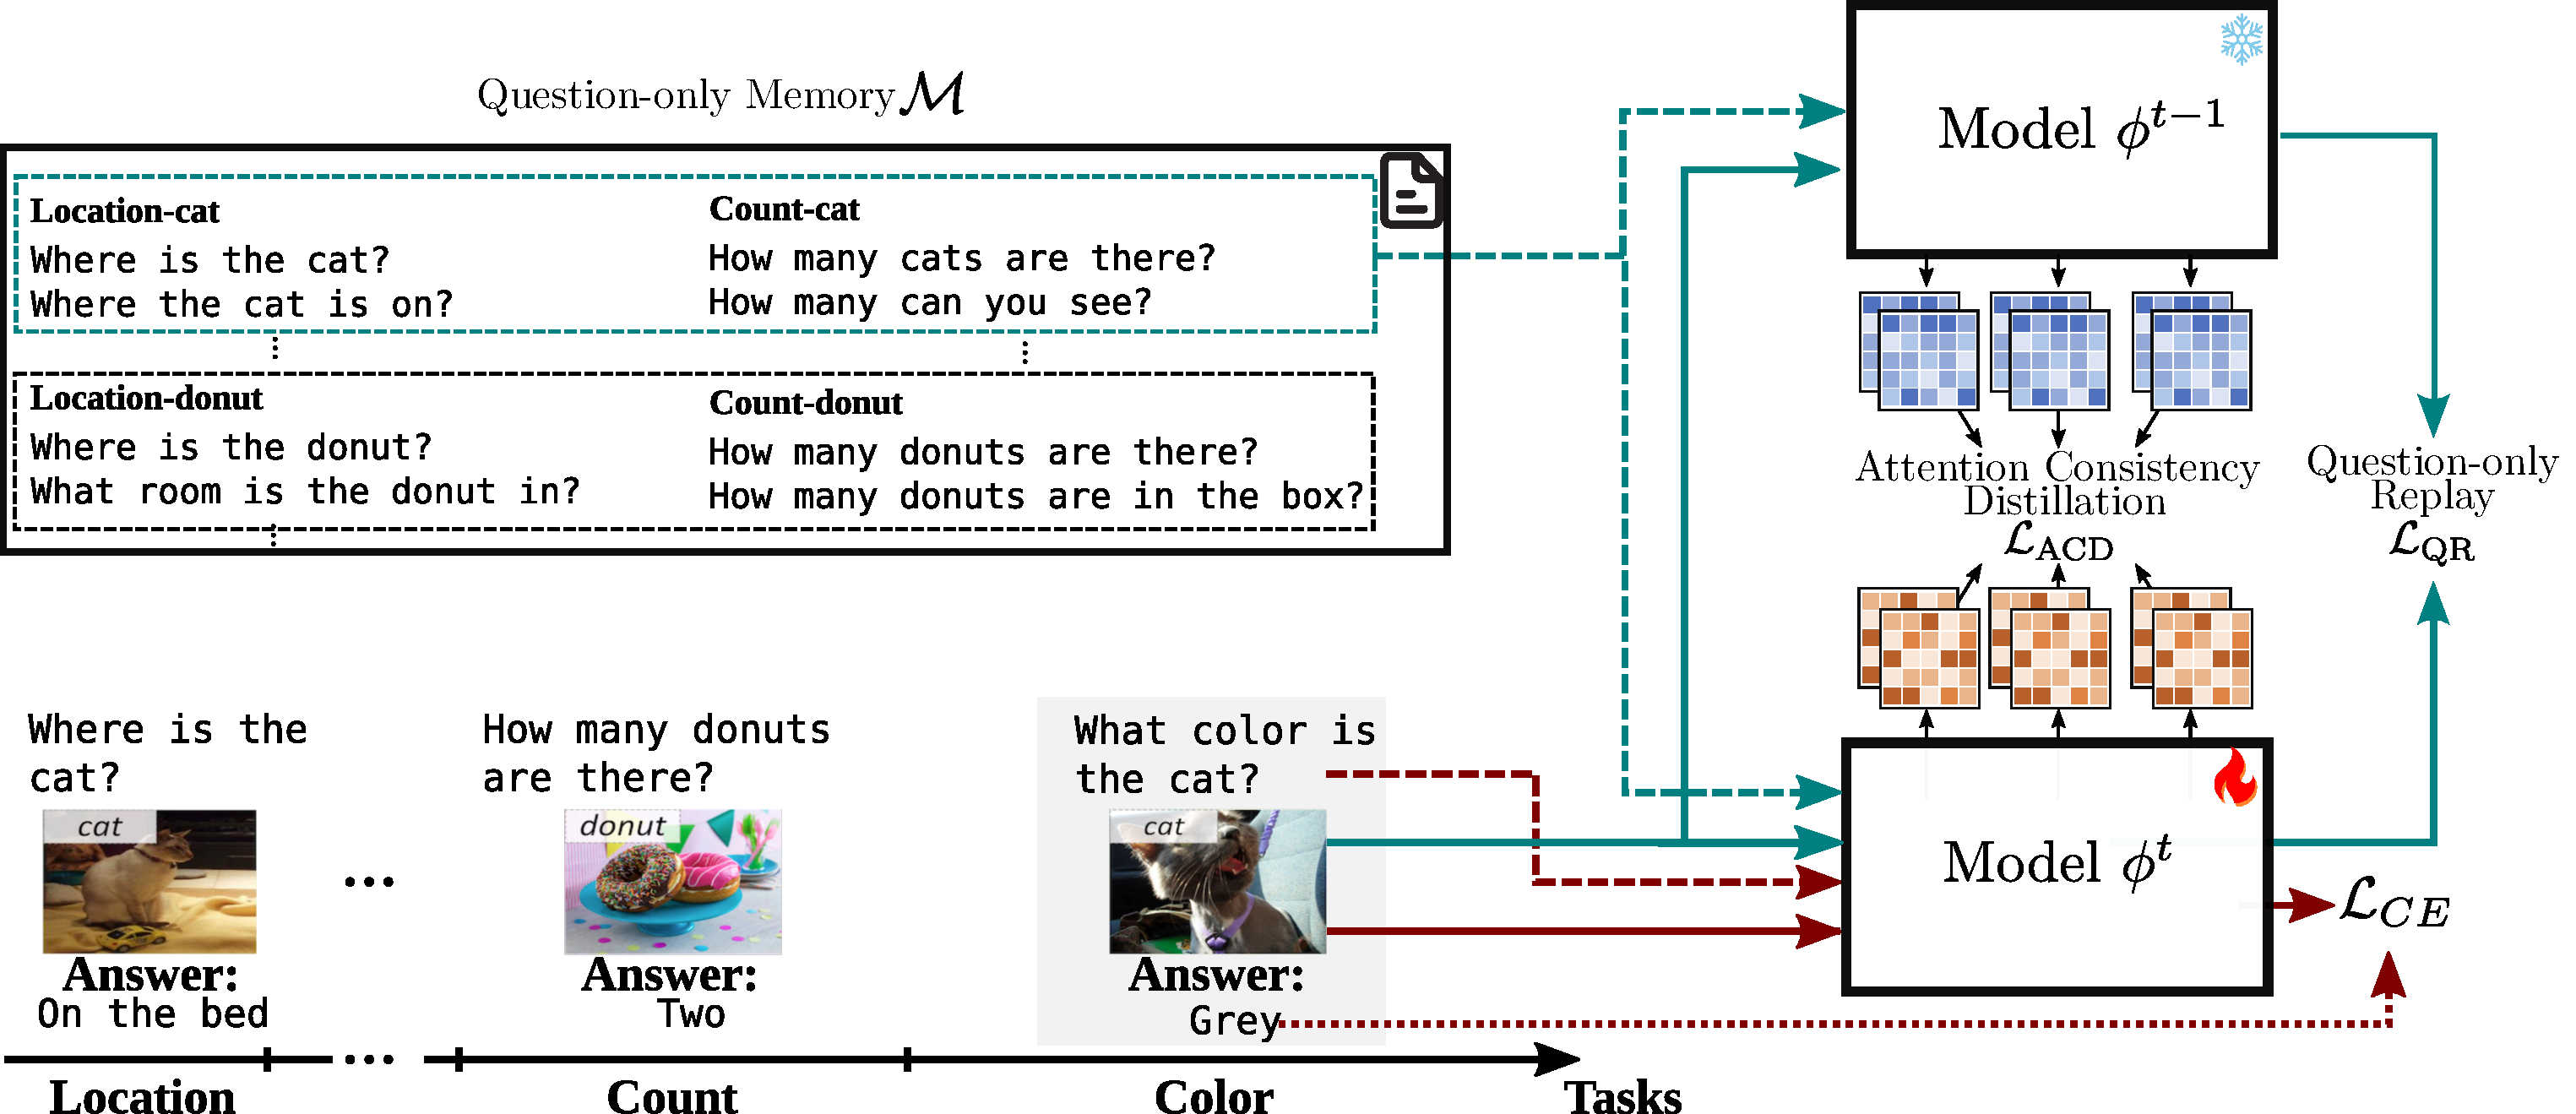
\includegraphics[width=0.85\linewidth]{Figures/method_quid.pdf}
    \caption{\textbf{Overview of \qstmethodshort{}}. 
    \qstmethodshort{} is composed of three components that jointly promote stability and plasticity in VQACL setting. 
    \textbf{(1) Question-Only Memory (\(\mathcal{M}\))} stores questions from past tasks, without visual data. \textbf{(2) Question-only replay} (\( \mathcal{L}_{\text{QR}} \)) leverages answers generated by the previous model \( \theta^{t-1} \) for new image-question pairs, encouraging the current model \( \theta^{t} \) to retain past knowledge. \textbf{(3) Attention Consistency Distillation} (\( \mathcal{L}_{\text{ACD}} \)) aligns the self-attention maps between \( \theta^{t-1} \) and \( \theta^{t} \) to maintain focus on relevant visual-linguistic relationships. 
    The task-specific loss (\( \mathcal{L}_{\text{CE}} \)) is applied solely to current task samples, promoting adaptation to new data.}
    \label{fig:main_fig}
\end{figure*} 

\subsection{Overview}
We propose \textbf{\qstmethodshort{}}, a novel approach for \setting{} framework that avoids image storage by relying solely on previously encountered questions (see Fig.~\ref{fig:main_fig}). Inspired by prior work in continual learning~\citep{li2017lwf, dhar2019learning}, we adopt a regularisation framework in which the overall learning objective $\mathcal{L}_{\text{VQACL}}$ is composed of two main components:
\begin{equation}
    \label{eq.trad_feat}
    \mathcal{L}_{\text{VQACL}} =  (1 - \lambda) \mathcal{L}_{\text{Plasticity}}+ \lambda\mathcal{L}_{\text{Stability}}.
\end{equation}
The plasticity term \(\mathcal{L}_{\text{Plasticity}}\), drives the model to adapt to the current task $\mathcal{T}^t$, while the weighting factor $\lambda>0$ balances the trade-off between the two loss terms.
Following common practice in VQA~\cite{zhang2023vqacl, Ravi_2023_WACV, Antol_2015_ICCV}, we implement the plasticity loss using cross-entropy to compare the network’s prediction for an input image-question pair \((x^t, q^t)\), against the ground-truth answer \(y^t\):
\begin{equation}
    \label{eq.trad_feat}
    \mathcal{L}_{\text{Plasticity}} = \mathbb{E}_{(x^t, q^t, y^t) \sim \mathcal{T}^t} \mathcal{L}_{\text{CE}}\left[\phi(x^t, q^t), y^t\right] .
\end{equation}
The second loss component, the stability term \(\mathcal{L}_{\text{Stability}}\), mitigates catastrophic forgetting. In the standard VQACL, where images from previous tasks are stored in memory \(\mathcal{M}\), the stability term is computed analogously using cross-entropy, averaging the loss over triplets \(~{(x^m, q^m, y^m) \in \mathcal{M}}\).
However, under the \setting~setting, storage of images \(x^m\) from past tasks in the memory \(\mathcal{M}\) is disallowed. To overcome this limitation, we design a novel stability loss \(\mathcal{L}_{\text{Stability}}\) tailored for \setting. Our approach integrates two complementary losses—question-only replay  $\mathcal{L}_{\text{QR}}$ and attention distillation $\mathcal{L}_{\text{ACD}}$—to effectively compensate for the absence of past task images, ensuring robust knowledge retention within the constraints of the \setting{} framework. Thus, the stability term is expressed as:
\begin{equation}
    \label{eq.trad_feat_stability}
    \mathcal{L}_{\text{Stability}} = \mathcal{L}_{\text{QR}}+\mathcal{L}_{\text{ACD}}.
\end{equation} 
Next, we describe the implementation of these loss components without storing past task images.
\subsection{Question-only Replay}%Pseudo-Labeling for 
To enhance knowledge retention in continual VQA, we propose a questions-only replay strategy that replays stored questions by pairing them with current task images to simulate past tasks. For each image from the current task $x^{t}$, we pair it with a question $q^{m}$ sampled from the memory. By combining stored questions with new images, our approach encourages the model to recall and reinforce previously acquired knowledge. Inspired by prior distillation-based works~\citep{li2017lwf, dhar2019learning}, we use the model from the previous task, $\phi^{t-1}$ to generate answers for each new image-question pair $(x^t, q^m)$. The generated answers act as soft pseudo-labels for the current model $\phi^{t}$, enforcing consistency with prior knowledge. The loss is defined as:
\begin{equation}
    \label{eq.trad_feat}
    \mathcal{L}_{\text{QR}} = \mathbb{E}_{x^t\sim \mathcal{T}^t}\mathbb{E}_{q^m\sim \mathcal{M}}\mathcal{L}_{\text{CE}}\left[\phi^{t}(x^t,q^m),\phi^{t-1}(x^t,q^m)\right].
\end{equation}
Notably, we employ the network’s output as soft pseudo-labels without applying the argmax operator. Using argmax would force the network to align exclusively with the most probable class; in contrast, soft pseudo-labeling allows for a more nuanced alignment with the full output distribution of $\phi^{t-1}$~\citep{hinton2015distilling, zhang2021refining, learning-soft-labels}.

These image-question pairs $(x^t,q^m)$ expose the model to a wide range of visual-question combinations, thereby improving the model’s retention of prior knowledge. Importantly, this strategy enables the model to maintain versatility in answering diverse question types, even when predictions exhibit some uncertainty. Without this regularization, the model becomes vulnerable to the \textit{out-of-answer-set problem}, wherein overfitting to the current task’s answer space results in erroneous responses for questions from prior tasks (see Fig.~\ref{fig.out_of_answer_set_problem}). For example, a model trained on color recognition might erroneously return a color name when confronted with a counting question from a previous task. Notably, this phenomenon closely resembles class recency bias in class-incremental learning (CIL), where models disproportionately favor newly learned classes over previously encountered ones ~\citep{rypesc2025task, mai2021supervised}.

\noindent\textbf{Question Selection for \qstmethodshort{}. }
Randomly pairing current task images \(x^{t}\) with past questions \(q^{m}\) from memory can partially mitigate forgetting but can produce semantically incoherent image-question pairs. 
For instance, if the current macro-task \(\mathcal{T}^t\) focuses on counting, naive pairing might associate an image of cars with the question ``\textit{How many cows are in this image?}'', leading to incoherent supervision and diminished performance. 
To address this, we introduce a targeted question selection strategy that prioritizes questions related to the object categories \(c_i\) in the current visually-driven subtask \(\mathcal{S}^l\). 
This ensures that replayed examples remain contextually meaningful, reinforcing relevant knowledge while preventing misleading associations. 
By aligning stored questions with the current task’s visual concepts, \qstmethodshort{} facilitates effective adaptation across linguistic and visual subtasks, improving continual learning performance.

\noindent \textit{Example:} Suppose the current visually-driven subtask 
$\mathcal{S}^t$ involves learning to count cars. The question selection strategy prioritizes memory questions relevant to cars, such as ``\textit{What’s the color of the car?}'', ensuring that replay maintains associations between visual and linguistic queries.

\subsection{Attention Consistency Distillation}
While question-only replay using pseudo-labeling ensures output consistency, it fails to constrain internal representations, causing self-attention drift and disrupting alignment with previously learned tasks~\citep{godey2024anisotropy, wang-etal-2022-learning, pelosin2022towards}. In contrast, feature distillation across multiple layers~\cite{Kang2022afc, xu2023multi,dhar2019learning, pelosin2022towards} offers stronger regularization by aligning internal representations; however, it often restricts plasticity due to its rigid constraints. These methods enforce layer-wise alignment, which becomes problematic when encountering new image-question pairs $(x^t, q^m)$ that were not present in previous training. Despite their semantic relevance, the model lacks prior exposure to these pairs, making strict layer-wise regularization overly restrictive. Our VQA model~\cite{zhang2023vqacl, nikandrou2022task} encodes image and text tokens within a unified transformer sequence, allowing self-attention to dynamically capture intra-modal (text-to-text, image-to-image) and inter-modal (text-to-image) dependencies. However, sequential fine-tuning gradually shifts self-attention~\cite{godey2024anisotropy, wang-etal-2022-learning}, causing the model to focus on different visual regions than those relevant to past tasks, ultimately degrading performance on prior knowledge~\cite{voita2019analyzing, godey2024anisotropy}. This drift arises because pseudo-labeling alone fails to stabilize internal representations, necessitating explicit regularization.

To mitigate this, we introduce \textit{attention consistency distillation} (ACD), which aligns the self-attention maps of the current model $\phi^t$ and its predecessor $\phi^{t-1}$. By preserving intra-modal and inter-modal relationships, this regularization stabilizes attention patterns while maintaining flexibility. Distilling only attention maps guides the model to attend to task-relevant visual regions for question answering while preserving adaptability to novel input patterns.

For an image-question pair $(x^t, q^m)$ with $x^t \sim \mathcal{T}^t, q^m \sim \mathcal{M}$: we denote \( A_k^t \) and \( A_k^{t-1} \) as the corresponding self-attention maps in an attention head $k$ for the current and previous model. Thus, we define the self-attention consistency loss $\mathcal{L}_{\text{ACD}}$ via cross-entropy, ensuring that attention distributions remain aligned across tasks:
\begin{equation}
\begin{split}
  \mathcal{L}_{\text{ACD}} = \mathbb{E}_{x^t\sim \mathcal{T}^t}\mathbb{E}_{q^m\sim \mathcal{M}}&\mathbb{E}_{k\sim \mathcal{K}_\phi}\\
  &\mathcal{L}_{\text{CE}}\left[A_{k}^{t}(x^t,q^m),A_{k}^{t-1}(x^t,q^m)\right],
\end{split}
\end{equation}
where $\mathcal{K}_\phi$ represents all attention heads across layers of $\phi$.

Unlike prior L1-based approaches~\citep{dhar2019learning, pelosin2022towards}, which impose uniform penalties and operate directly on the raw query-key products, ACD leverages cross-entropy on normalized attention maps (after softmax operation) to preserve the probabilistic structure of attention distributions. This gives greater emphasis to highly attended regions while low-attended areas remain flexible, preventing over-penalization of less critical regions. Asymmetric regularization (e.g., ReLU+L1) ~\citep{pelosin2022towards} partially addresses this issue by prioritizing reductions in attended regions but lacks a probabilistic alignment mechanism, making it less effective in maintaining structured dependencies in multimodal learning. In contrast, ACD offers an importance-weighted alignment that preserves essential cross-modal associations without hindering adaptation. The effectiveness of ACD is empirically demonstrated in Sec.~\ref{sec:experiments}, and further discussed in the Appendix.

\input{sec/tables/main_tab}
